\documentclass{standalone}

\usepackage[dvipdfmx]{graphicx}
\usepackage{tikz}


\begin{document}

\begin{tabular}{c|cc}
Step & Script buffers & Gola window \\\hline
0 & 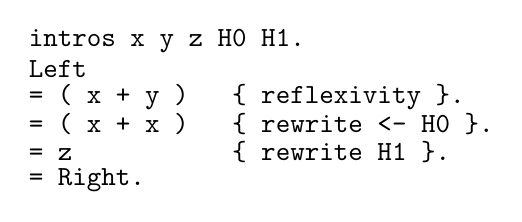
\begin{tikzpicture}[
  baseline=(T.base),
  high_light/.style={circle, rectangle, minimum size = 10pt, inner sep=0pt, fill=lightgray},
  non_high_light/.style={circle, rectangle, minimum size = 10pt, inner sep=0pt},
]
\draw (0,0) node (T) [non_high_light, right] {\verb-intros x y z H0 H1.-};
\draw (0,-10pt) node [non_high_light, right] {\verb-Left-};
\draw (0,-20pt) node [non_high_light, right] {\verb-= ( x + y )   { reflexivity }.-};
\draw (0,-30pt) node [non_high_light, right] {\verb~= ( x + x )   { rewrite <- H0 }.~};
\draw (0,-40pt) node [non_high_light, right] {\verb-= z           { rewrite H1 }.-};
\draw (0,-50pt) node [non_high_light, right] {\verb-= Right.-};
\end{tikzpicture} & \begin{minipage}[t]{140pt}\footnotesize
\begin{verbatim}
============================
forall x y z : nat,
x = y -> z = x + x -> x + y = 
\end{verbatim}
\end{minipage}\\\hline
1 &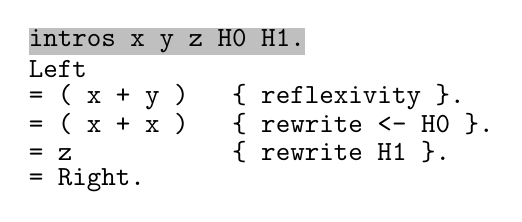
\begin{tikzpicture}[
  baseline=(T.base),
  high_light/.style={circle, rectangle, minimum size = 10pt, inner sep=0pt, fill=lightgray},
  non_high_light/.style={circle, rectangle, minimum size = 10pt, inner sep=0pt},
]
\draw (0,0) node (T) [high_light, right] {\verb-intros x y z H0 H1.-};
\draw (0,-10pt) node [non_high_light, right] {\verb-Left-};
\draw (0,-20pt) node [non_high_light, right] {\verb-= ( x + y )   { reflexivity }.-};
\draw (0,-30pt) node [non_high_light, right] {\verb~= ( x + x )   { rewrite <- H0 }.~};
\draw (0,-40pt) node [non_high_light, right] {\verb-= z           { rewrite H1 }.-};
\draw (0,-50pt) node [non_high_light, right] {\verb-= Right.-};
\end{tikzpicture} & \begin{minipage}[t]{140pt}\footnotesize
\begin{verbatim}
x, y, z : nat
H0 : x = y
H1 : z = x + x
============================
x + y = z
\end{verbatim}
\end{minipage}\\\hline
2 &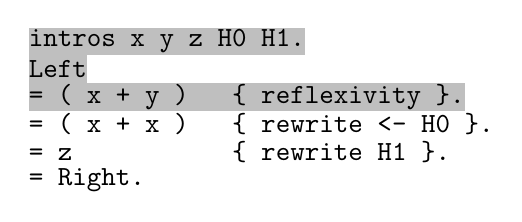
\begin{tikzpicture}[
  baseline=(T.base),
  high_light/.style={circle, rectangle, minimum size = 10pt, inner sep=0pt, fill=lightgray},
  non_high_light/.style={circle, rectangle, minimum size = 10pt, inner sep=0pt},
]
\draw (0,0) node (T) [high_light, right] {\verb-intros x y z H0 H1.-};
\draw (0,-10pt) node [high_light, right] {\verb-Left-};
\draw (0,-20pt) node [high_light, right] {\verb-= ( x + y )   { reflexivity }.-};
\draw (0,-30pt) node [non_high_light, right] {\verb~= ( x + x )   { rewrite <- H0 }.~};
\draw (0,-40pt) node [non_high_light, right] {\verb-= z           { rewrite H1 }.-};
\draw (0,-50pt) node [non_high_light, right] {\verb-= Right.-};
\end{tikzpicture} & \begin{minipage}[t]{140pt}\footnotesize
\begin{verbatim}
x, y, z : nat
H0 : x = y
H1 : z = x + x
d := direction Rightwards : Prop
============================
x + y = z
\end{verbatim}
\end{minipage}\\\hline
3 &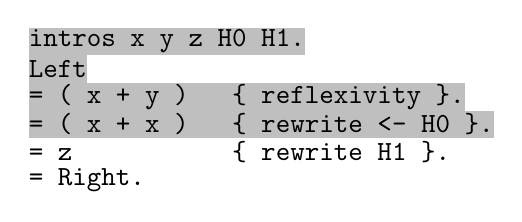
\begin{tikzpicture}[
  baseline=(T.base),
  high_light/.style={circle, rectangle, minimum size = 10pt, inner sep=0pt, fill=lightgray},
  non_high_light/.style={circle, rectangle, minimum size = 10pt, inner sep=0pt},
]
\draw (0,0) node (T) [high_light, right] {\verb-intros x y z H0 H1.-};
\draw (0,-10pt) node [high_light, right] {\verb-Left-};
\draw (0,-20pt) node [high_light, right] {\verb-= ( x + y )   { reflexivity }.-};
\draw (0,-30pt) node [high_light, right] {\verb~= ( x + x )   { rewrite <- H0 }.~};
\draw (0,-40pt) node [non_high_light, right] {\verb-= z           { rewrite H1 }.-};
\draw (0,-50pt) node [non_high_light, right] {\verb-= Right.-};
\end{tikzpicture} & \begin{minipage}[t]{140pt}\footnotesize
\begin{verbatim}
x, y, z : nat
H0 : x = y
H1 : z = x + x
d := direction Rightwards : Prop
============================
x + x = z

\end{verbatim}
\end{minipage}\\\hline
4 &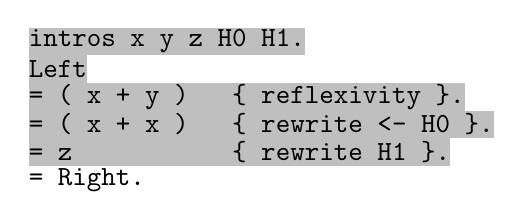
\begin{tikzpicture}[
  baseline=(T.base),
  high_light/.style={circle, rectangle, minimum size = 10pt, inner sep=0pt, fill=lightgray},
  non_high_light/.style={circle, rectangle, minimum size = 10pt, inner sep=0pt},
]
\draw (0,0) node (T) [high_light, right] {\verb-intros x y z H0 H1.-};
\draw (0,-10pt) node [high_light, right] {\verb-Left-};
\draw (0,-20pt) node [high_light, right] {\verb-= ( x + y )   { reflexivity }.-};
\draw (0,-30pt) node [high_light, right] {\verb~= ( x + x )   { rewrite <- H0 }.~};
\draw (0,-40pt) node [high_light, right] {\verb-= z           { rewrite H1 }.-};
\draw (0,-50pt) node [non_high_light, right] {\verb-= Right.-};
\end{tikzpicture}&\begin{minipage}[t]{140pt}\footnotesize
\begin{verbatim}
x, y, z : nat
H0 : x = y
H1 : z = x + x
d := direction Rightwards : Prop
============================
z = z
\end{verbatim}
\end{minipage}\\\hline
5 &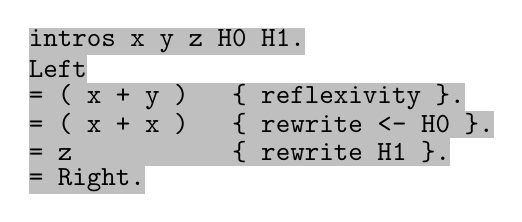
\begin{tikzpicture}[
  baseline=(T.base),
  high_light/.style={circle, rectangle, minimum size = 10pt, inner sep=0pt, fill=lightgray},
  non_high_light/.style={circle, rectangle, minimum size = 10pt, inner sep=0pt},
]
\draw (0,0) node (T) [high_light, right] {\verb-intros x y z H0 H1.-};
\draw (0,-10pt) node [high_light, right] {\verb-Left-};
\draw (0,-20pt) node [high_light, right] {\verb-= ( x + y )   { reflexivity }.-};
\draw (0,-30pt) node [high_light, right] {\verb~= ( x + x )   { rewrite <- H0 }.~};
\draw (0,-40pt) node [high_light, right] {\verb-= z           { rewrite H1 }.-};
\draw (0,-50pt) node [high_light, right] {\verb-= Right.-};
\end{tikzpicture}&
\end{tabular}
\end{document}

